\chapter{Protocol Translation}
\label{sec:imperative_form}

The task of the Reo compiler is to translate a Reo protocol specification into the target language. The resulting code must interface with other components written in the language such that, at runtime, the resulting system behaves as specified. In this chapter, we explain how we extend the Reo compiler to support the Rust language target.

Section~\ref{sec:two_phase} examines the task of the backend, the translation from the Reo compiler's internal representation (`RIR') to an executable protocol object in the target language. This task is broken down into smaller, more specialized subtasks. Section~\ref{sec:decoupling_reo_rust} organizes these subtasks into a pipeline that sees the translation through from Reo specification to executable Rust protocol object. To bridge the gap between Reo and Rust compilers, Section~\ref{sec:imperative_form_sec} defines \textit{imperative form} (`IF') as a novel representation of a protocol's behavior in a manner conducive to imperative languages, but not yet fine-grained or inherently coupled to one language in particular. Section~\ref{sec:translation_pipeline} goes into detail about the implementation of the translation pipeline by explaining how the previously-defined subtasks are completed in stages. This includes an example of the output of the Reo compiler: Rust source code whose contents are primarily a Rust-embedded representation of IF.

%\hl{
%	The task of the Reo compiler is to translate a Reo protocol specification into the target language. The resulting code must interface with other components written in the language such that, at runtime, the resulting system behaves as specified. Rust is an example of an imperative language, unable to represent port interactions at the same high level. Our generated code must implement the specification in terms of imperative actions
%	
%	Imperative languages must instead 
%	between a set of \textit{components} written in the target language. When connected together in the manner corresponding to the s
%	
%	the task is to generate a rust protocol object from the reo spec such that it can be used in a rust program.
%	3. naive extreme: 100 percent reo is infeasible: must do signficiant work emulating rust. and they both become tightly coupled
%	4. java solution is to move common object defs to a library. this is fine but its not enough! (WHY)
%	5. 
%	4. java recognized this problem and has the solution of using a lib for protocol and port. still, if we attempted to emulate this choice of granulairty, reo would still do the majority of the heavy lifting
%	5. we have a structured approach. isolate the tasks involved in the transformation. we identify that two are language-independent if beyond the target being imperative. 
%	6. we make this distinction concrete in considering it a two-step process with imperative form in the middle: representing the specification of an imperative protocol.
%	
%	3. follow the precedent of moving as much as possible to a library. minimizes repetition and avoids reo compiler from being too coupled on the implementation. on the other hand, moving things into the library prevent them from being entirely statically generated; forces us to express it in terms that can be computed at runtime. we strike a balance by performing all the high level transformations at runtime 
%}

%In this chapter, we describe the process of translating the Reo compiler's internal representation of a protocol specification into an executable \textit{protocol object} in the Rust language.

\section{Structuring the Translation Process}
\label{sec:two_phase}
In this section, we explore the nature of the task which characterizes the Rust backend for the Reo compiler. Section~\ref{sec:sub_tasks} breaks the problem down into simpler subtasks, and explains their relationship to one another and how they apply in the case of a different target language. Section~\ref{sec:decoupling_reo_rust} explains how these tasks are organized by defining their place within a translation pipeline. The implementation of the pipeline itself is given in Section~\ref{sec:translation_pipeline}.

\subsection{Translation Subtasks}
\label{sec:sub_tasks}
The Reo compiler's frontend parses its input in the Reo language with textual syntax. It performs significant transformations on its internal representation before arriving at what we call RIR. Everything that follows is the task of the backend, transforming it further until code in the target language can be emitted. Reo and Rust differ significantly in how they represent work. Accordingly, a protocol expressed in the former must be transformed significantly before it can be expressed in the latter. In this section, this task is decomposed into \textit{subtasks} which serve a dual purpose (1) smaller tasks are more easily understood, and help to characterize Reo and Rust by identifying their differences, and (2)~only isolated subtasks can be separated, allowing the entire task to be performed in stages, as the \textit{pipeline}.  Here, we explain how the pipeline is structured; the implementation of the subtasks is left to Section~\ref{sec:translation_pipeline}.

\subsubsection{Input Representation}
RIR embodies the completion of several of the operations on Reo connectors described in the literature~\cite{baier2006modeling, dokter2018rule}; namely, \textit{composition}, \textit{merging}, \textit{hiding}, and so on. For our purposes, it suffices to say that RIR is presented in a form corresponding closely to an RBA, one of the semantic models described in Section~\ref{sec:semantic_models}. RIR is self-contained, and defines a list of \textit{rules} which correspond 1-to-1 to interactions between the protocol's ports. It captures the intuition of an RBA as they are usually understood in an imperative context; rules are subdivided into parts \textit{guard} and \textit{assignment}. Helpfully, RIR presents the latter not as a monolithic formula, but rather as a mapping from identifier to \code{Term} objects. In our imperative context, terms can be understood as expressions to be evaluated at runtime. For example, \code{True} is a boolean type term, while \code{Port("A")} may be understood as the value put by port~$A$.

\subsubsection{Subtasks Involving Actions and Data Types}
Reo specifications represent connectors declaratively as relations between ports. They are thus well suited to reasoning about the protocol's properties. In contrast, our target imperative languages such as Java and Rust represent computation such that it corresponds more closely to machine instructions; they are \textit{imperative}, laying out sequences of actions which together emerge as interaction at runtime. Where interactions in the former can be oriented around the synchronous observations of port values, interactions of the latter must be expressed as sequences of actions, laid out over time. RIR is somewhere in between. Per RIR rule, the guard is distinguished from the assignment, suggesting a coarse-grained ordering of operations: the guard is evaluated before values are assigned. This is a step in the right direction, but requires further transformation before it can correspond to executable Rust. For example, RIR is able to disambiguate the order in which memory cells are read and written to by implying an ordering by annotating their identifiers with qualifiers comparable to those in temporal logic (in both syntax and semantics). For example, the assignment corresponding to $m=A\wedge{}m'=B$ does not explicitly express an ordering, but nevertheless implies it by annotating $m$ with a qualifier to represent its `next' value. Rust's imperative nature requires that operations on values occur in the order of their appearance in the program's control flow, as this determines the order in which they will be executed (Rust compiler optimizations aside).

Java, Rust and Reo have in common that they are strongly-typed languages. In the broader sense, `type' describes the classification of just about everything in Reo, including connectors and primitives. The Reo compiler's internals perform transformations that handle the majority of what could be considered `type checking'. The only exceptions are (1) the data types of each port, determining the types of values they transmit, and (2) the types of functions applied to values within the channel, which are expressed as relations between an identifier and a list of arguments (each expressed as \code{Term}). For the sake of programmer ergonomics, Reo permits the data types of ports to be omitted, such that they can later be derived in context. As this task is not performed by the Reo compiler's frontend, it becomes the responsibility of the backend to resolve these types. In compiling to Rust, the backend must take care that these types adhere to Rust's rules for types as well as Reo's. For imperative languages without types, it suffices to represent them with a universal type, e.g., \code{Object} in Java.

\subsubsection{Subtasks for Abstract and Concrete Targets}
Regardless of any intermediate representation, protocols must ultimately be emitted in the target language at the required level of specificity. Imperative languages place the burden of defining \textit{how} their work is performed squarely on the shoulders on the programmer. For example, where a declarative language might not distinguish \textit{merge sort} from \textit{bubble sort}, Rust certainly does; a Rust program's operations on variables correspond (relatively) closely to machine instructions as they will be executed at runtime. This is also true in the case of our problem; what is implied in Reo must be made explicit in Rust. This includes the initialization of system resources, operations on concurrency primitives, and all the minutia necessary to implement the optimizations described in Section~\ref{sec:behavior_implementation}. 

We observe that one can perform meaningful protocol translation work, resulting in its expression in imperative manner without committing to a particular language's minutia. On the other hand, an abstract specification may be made concrete by translating it into a particular language. We distinguish these notions by differentiating between specification and implementation.\footnote{These abstract concepts tend to fall apart under scrutiny, as they depend on what is meant by `computation' at all. Nevertheless, this observation is helpful in the context of our problem, as we prescribe the relationship between Reo and Rust by using the former to `model' the latter.}  

It is beneficial to recognize that a significant portion of the translation from Reo to Rust would be shared by the same procedure to a similar language; the more similar the language, the more we can expect their respective transformations to have in common. For example, despite their significant differences, Rust and Java are more similar to each other than they are to Reo. We attempt to generalize Rust, Java and languages like them in accordance with common terminology. We characterize \textit{imperative} languages by a need to make explicit their \textit{control flow} by imposing a total order on their actions. Recall the example of a memory cell, for which both a read and a write are expressed as part of an interaction $m=A\wedge{}m'=B$. An imperative language would require that these two distinct actions be laid out in a sequence: namely, $[m=A, m=B]$. Observe that with the order made explicit, the temporal (`next') qualifier can be discarded without introducing ambiguity.

Toward compilation to Rust, we are forced to resolve the data types of ports and functions. This resolution is a property of Reo itself, which has its own notion of port data types. For this reason, we are able to reason about the \textit{properties} that characterize a port type, insofaras the releation is meaningful to Reo itself (and not introduced only when implementing the protocol). For example, we may reason that a ports type must facilitate its values being \textit{replicated} if an interaction exists that replicates a value of its type. However, Reo does not prescribe what these types are called in the target language, nor does it prescribe any additional relationships between them. For example, two types distinguished by Reo may be unified in implementation. 

In the sequel, we consider translation work \textit{abstract} if is produces a representation valuable to any imperative language, and \textit{concrete} otherwise.


\subsubsection{Translation Subtasks Defined}

Ultimately, we partition the task of translating from RIR to Rust as four subtasks, where those that are \textit{abstract} precede those that are \textit{concrete}:

\begin{tabular}{l|p{5cm}p{5cm}}
	& Action & Data Type \\
	\hline
	Abstract & $T_{AA}$: From each abstract interaction, a sequence of imperative actions are laid out. & $T_{AT}$: Ports are mapped to data types characterized by properties. \\
	\hline
	Concrete & $T_{CA}$: Abstract actions are reified into concrete, executable Rust code. & $T_{CT}$: Abstract data types are resolved to satisfactory concrete Rust types.
\end{tabular}


\subsection{Pipelining Subtasks}
\label{sec:decoupling_reo_rust}

Code generation is an unusual problem, as it introduces a spectrum of possibilities in response to questions that usually have trivial answers. For example, in which language is a concept expressed? Reo specifies the coordination behavior of the generated Rust code, but (by design) nothing more. This freedom makes room for questions of `where' and `when' the behavior that emerges at runtime is made concrete. 

Toward an answer, we begin by considering one of the possible extremes: the Reo compiler performs as much of the work (i.e., as many of the subtasks) as possible. Whatever behavior is desired in the executable program is spelled out in detail, and reflected explicitly in the Rust code the Reo compiler produces. This solution is arguably the most intuitive, and it has many advantages. For example, we are able to `front-load' as much computation work as possible, such that the generated Rust code can represent operations in a preprocessed form. We are also given fine control over the behavior of the final binary. However, this strength is what makes this approach impractical: the Reo compiler's ability to specify Rust's behavior in detail also implies a responsibility to do so. By reasoning about the Rust-compiled program directly, Reo must model Rust's language and tooling environment. Recreating this existing work is a poor use of the available software resources. Worse still, it results in Reo compiler becoming tightly coupled to the Rust language, not only syntactically, but in the fine-grained logic necessary for implementing our desired performance optimizations in full detail. At the same time, all flexibility is taken away from the user; they have no ability to understand or influence the concrete implementation themselves. Essentially, this approach trivializes the contributions of Rust compiler.

As one might expect, the opposite extreme trivializes the contributions of the Reo compiler. If hardly any transformations at all are applied before Rust code is emitted, the representation can only be very similar to that of RIR. As explained previously, these forms are simply too different for the Rust compiler to use as-is. By necessity, either a new Rusty-RIR to Rust translation tool would have to be introduced, or the translation would have to occur inside the Rust-generated program at runtime. Either way, the work of performing our abstract transformations is simply postponed to later stage in the pipeline.

Between these extremes there is a vast spectrum. Ultimately, we wish to choose a balance that partitions the work between the compilers of Reo and Rust in a manner that befits the interests of the language, minimizing the extent to which Reo models Rust or vice versa. Section~\ref{sec:sub_tasks} touched on the observation that a portion of the work in translating from RIR to Rust is common to other imperative language targets. Our solution is for the Reo compiler to perform only the `abstract' subtasks ($T_{AA}$, $T_{AT}$), translating RIR to a form for which imperative computation is natural, but is otherwise as agnostic to the target language as possible. Reo emits abstract behavior for the Rust compiler to make concrete. Clearly, this abstract representation must be understood by both Reo and Rust compilers, as it crosses the boundary between their stages in the pipeline. To follow, Section~\ref{sec:imperative_form_sec} defines this representation as \textit{imperative form}, embodying the behavior of an abstract imperative language.

Clearly, the Reo compiler backend itself performs the abstract subtasks, but what exactly performs the concrete subtasks?
The Reo compiler has an existing backend for generating Java code. It works by generating Java according to the structure of a \textit{template generator}, which defines a hierarchy of string macros for formatting RIR objects in Java's syntax. At first glance, this backend exemplifies the extreme of Reo modeling the target language, performing all of the subtasks itself. However, the extent of the associated coupling to Java is mitigated through the reliance on a purpose-built Java library. Within, definitions are provided for objects that all Reo-generated Java programs will have in common. For example, the library defines a \code{Component} interface, for which the code generator produces a protocol-specific implementor class. This approach works to minimize the `surface' of the generated code, by having Reo generate behavior at a higher level of abstraction. Reo generates Java in Java-specific terms, but must generate less overall.

Our approach follows the precedent set by the Java backend; we introduce \textit{Reo-rs}, a purpose-built Rust library which reduces the Rust-specific surface exposed to the Reo compiler. Specifically, Reo-rs defines types that `hide' their Rust-specific complexities behind an abstract API. We reduce the burden on the Reo compiler further by reducing the granularity of the protocol representation as it appears in the Rust source code; the Reo compiler emits a single \code{entrypoint} function, which acts as a thin wrapper around the initialization of a \code{ProtoDef}. This structure is provided by Reo-rs, and corresponds with IF, as it is defined in Section~\ref{sec:imperative_form_sec}. By expressing the protocol's behavior in this form, the Reo compiler takes responsibility only of the abstract transformation steps: $T_{AA}$ and $T_{AT}$. Rust itself completes the translation to its language specifics, partly at compile time and partly at run time. Figure~\ref{fig:pipeline} gives an overview of the entire process from start to finish, ultimately resulting in objects which coordinate the components of a program written in the Rust language. Section~\ref{sec:translation_pipeline} explains the implementation of these stages, and their relationships in more detail.

\begin{figure}
	\centering
	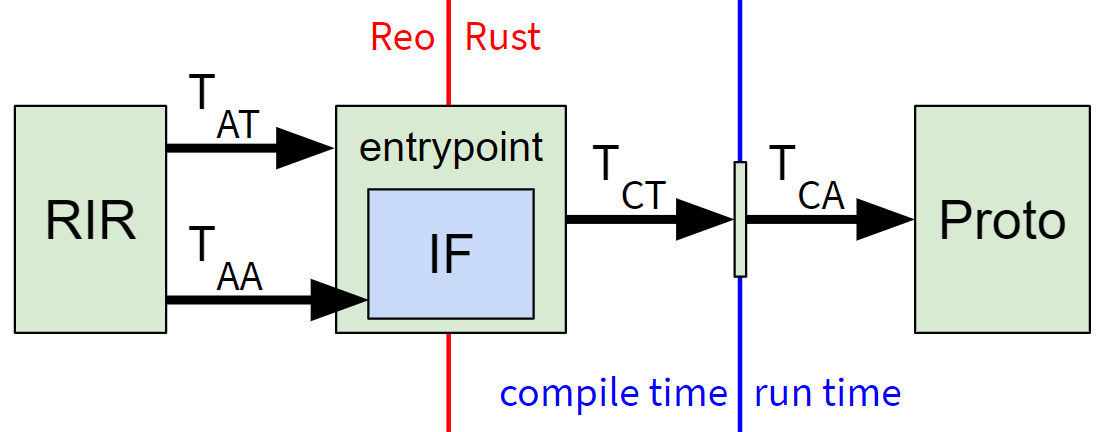
\includegraphics[width=0.67\textwidth]{pipeline.png}
	\caption[Reo to Rust code generation pipeline.]{The translation pipeline from the Reo compiler's internal representation (`RIR') to the executable Rust \code{Proto} object. Translation phases correspond to subtasks defined in Section~\ref{sec:sub_tasks}. The majority of the specification is represented in the imperative form (`IF'), which serves as the representation at the boundary between Reo and Rust. The boundary between compile and run time is relative to that of the user's Reo-coordinated program.}
	\label{fig:pipeline}
\end{figure}

\subsection{Enabling Future Expansion}
Previously, we observed that the translation work from Reo to its targets can be expected to have significant overlap. For our purposes, we characterize imperative languages by defining IF in Section~\ref{sec:imperative_form_sec}, and build our translation pipeline around its use as an intermediate representation.

Performing the translation in clear stages is beneficial to both Reo and its target languages. The benefits to new targets is clear; they may acquire Reo support with less effort than otherwise. Existing target languages are able to benefit also, as they are able to implement the same IF using different concrete translation procedures, i.e., they may implement $T_{CA}$ and $T_{CT}$ differently. Regardless of concrete implementation, protocol objects stemming with an IF specification in common are safe in the knowledge that they will agree on their abstract action sequences, and the abstract types of their ports.

For the sake of limiting the scope of the project, we relegate IF to a tool unique to the generation of the Rust language; as far as the user is concerned, the Rust backend emits Rust directly, which they are able to use as part of their Rust programs. Future work may remove this restriction by having Reo support IF as a compilation target directly. For a more detailed discussion, see Section~\ref{sec:future_imperative_compiler}.

\section{Imperative Form}
\label{sec:imperative_form_sec}
In this section, we define \textit{imperative form}, a novel intermediate representation of the behavior of Reo protocols, such that they more closely correspond to their final representation in some imperative language. In the protocol translation pipeline, this form is the result of completing translation subtasks $T_{AA}$ and $T_{AT}$, as they are defined in Section~\ref{sec:sub_tasks}. At this stage, we take for granted that ports and functions have been given abstract types by the Reo compiler.

\subsection{Concept}
RIR does not ergonomically facilitate execution, primarily because it does not define the \textit{order} in which values are accessed, created and moved. Programmers using imperative, sequential languages are very used to thinking in terms of procedures which manipulate the state of variables \textit{in scope} with the order of actions expressed as the control flow. Often, interpreters or compilers provide safety properties by tracing over the control flow, and emitting errors whenever a variable access is invalid.

IF makes explicit the ordering between symbolic \textit{actions}; if executed in the specified order, it is guaranteed that (1) variable accesses are always valid, and (2) a rule fires unambiguously; the effects of a rules actions are only observable if and only if the rule has fired.

\subsubsection{Rules as Transactions}

RIR partitions the work of a rule into its \textit{guard} and \textit{assignments}. This is already a step in the direction of imperative computation, observing that some work (the guard) must be performed prior to deciding whether the rule fires, in which case the assignment follows. As the protocol does not define the moments when it will evaluate the guard, it is an error to define a guard whose evaluation `leaks' meaningful behavior. 

We are able to interpret a RIR rule as a two-action \textit{transaction} which \textit{commits} after the first, guaranteeing the second will occur. Prior to the moment of commitment, actions are (1) obligated to have a defined means of being \textit{reversed}, undoing their observable effects on the environment, leaving no trace of their execution, and (2) able to initiate an \textit{abort}, reversing their effects. In this view, the guard's evaluation instigates an abort if it evaluates to $false$.

IF adopts the notion of ordered actions from RIR, but generalizes it to a sequence of any length of at least one. For our purposes, it suffices to have a fixed moment of commitment: immediately before the last action. Accordingly, we retain the term `assignment' for this last action to mirror RIR. All other actions are transient, and behave as described above. One final stipulation is needed: after an action's effects are reversed, its predecessor action is reversed also (if they exist). Consequently, an abort propagates up through the transient actions in the opposite order they were originally performed, reversing all of their effects on the state one by one. However, once the last action is reached, the rule's firing has committed, and the effects of all actions will be observed.

\subsubsection{Action Granularity}
IF represents a protocol's defined interaction as actions to be computed in the specified sequence. At this stage, our representation is still symbolic; actions do not necessarily correspond 1-to-1 with concrete operations in the target imperative language, and their representation of actions is unspecified as long as they preserve the properties of IF. We represent actions at the coarsest granularity possible to avoid overspecifying the ordering of concurrent operations by leaving for meaningful implementation choices in subtask $T_{CA}$.

The simplest IF rules can be represented with a single action; implicitly, the rule has a trivial guard (consisting of zero actions), consisting entirely of some guaranteed assignment. For example, a rule with a trivial data constraint may be represented as a single, trivial action; the rule always fires to no effect.

The utility of our generalization is the ability to break up a single action into multiple in a manner we are able to represent. For example, we are able to reason about actions that create \textit{temporary variables}, corresponding to the creation of new values at runtime. These actions may be transient, as reversal is easily defined: discard the value. To illustrate our ability to split actions, we represent a protocol, expressed in RBF with data constraint $X=f(X)$ and synchronization constraint $\{X\}$ with only input (putter) port~$P$. This rule can be understood as ``$X$ fires if and only if the results of function~$f$ on its put value is equivalent to the value itself''. Here, the result of $f$ clearly cannot be inspected until \textit{after} it is computed. We are able to represent this rule with an action sequence of length three: (1) Create temporary value $f_X$ by executing $f$ given argument $X$. (2) Trigger an abort if $f_X\neq{}X$. (3) The rule has fired; do nothing other discarding values $X$ and $f_X$. 


\subsection{Definition}
\label{sec:imperative_form_definition}
Here we define \textit{imperative form}, and explain how its definition corresponds with the intuition behind it. Firstly, an IF contains a structure which corresponds to a \textit{symbol table}; this does the work of assigning symbolic \textit{data types} to ports and memory cells. Ports must also be annotated with an explicit \textit{orientation} (i.e.,\ input or output). Other symbols are also represented here, for example, the names and the argument types for any named functions.

More interesting are the \textit{imperative rules} listed for an IF, corresponding to rules of an RBA or RBF. Each rule is given by a tuple $(P,I,M)$ where:
\begin{enumerate}
	\item \textbf{Premise $P$}\\
	The premise is another tuple of three \textit{identifier} sets $(P_R, P_F, P_E)$. $P_R$~is the \textit{synchronization constraint}, i.e.,\ the set of ports identifiers whose values must be `ready'. $P_F$ and $P_E$ are the sets of \textit{memory values} which must be known to be full and empty respectively, such that it is known whether they can be read from or written to. The rule can certainly not consider firing unless all ports are ready and all memory cells are in the specified states.
	
	\item \textbf{Instructions $I$}\\
	A list of reversible \textit{instructions} which are performed in sequence. These instructions have no immediately observable effects, such that they can be reverted in the event of an \textit{abort}. Concretely, each instruction is one of:
	\begin{itemize}
		\item $check(p)$\\
		Trigger an \textit{abort} if predicate $p$ over data is satisfied.
		\item $fill_P(m, p)$\\Fill an empty memory variable $m$ with the result of a predicate $p$ over available data. The value's data type is implicitly \textit{boolean}.
		\item $fill_F(m, f, a)$\\
		Fill an empty memory variable $m$ with the result of invoking function $f$ with arguments $a$, a list of references to value identifiers with length matching the arity of $f$. It is incorrect for $f$ to \textit{mutate} the values of its arguments, as this would result in observable effects which cannot be rolled back.
		\item $swap(m_0,m_1)$\\
		Swap the values in two memory variables~$m_0$ and~$m_1$.
	\end{itemize}
	If an abort is triggered by $check$, any swapped memory cells are swapped back, and any memory cells whose values were created by $fill_P$ or $fill_F$ are destroyed.
	
	\item \textbf{Movements $M$}\\
	A mapping from identifiers of \textit{values} to the identifiers of getter ports and empty memory cells (`destinations'). This represents the final action of an imperative rule executed if and only if the rule \textit{fires}.
\end{enumerate}

An imperative rule aims to model a sequential computation from top to bottom. Instructions are able to (non-destructively) read values, create new variables, and swap the values of variables. Starting from the premise, one is able to populate a set of values' identifiers \textit{in scope}, and then traverse the instructions and rules. For this reason, it is beneficial to distinguish $P$ from an instruction: $P$ also establishes the initial scope.

The IF is well-formed only if no instruction no the movement is \textit{invalid}. Here, it suffices to say that validity models the usual scoping rules in an imperative language. For example, one cannot read from an uninitialized value. Other restrictions are in place to ensure that instructions are always reversible. For example, $fill_F$ may only be used if the value it populates is previously uninitialized. The full enumeration of constraints is available in the source code, visible in the \code{build} function of the \code{ProtoDef} type (this is explained further in Section~\ref{sec:translation_phase_2}, including a listing with some example errors).

$M$ is defined with a representation that makes it trivial to distinguish the cases where values are discarded (0 destinations), moved linearly (1 destination) or replicated (multiple destinations). This design is convenient for languages that require their values to be more explicitly managed. For example, languages with \textit{affine types} (e.g.,\ Rust) must simulate the replication of values by creating new affine resources from the original, and managing the replicas explicitly.  \textit{Relevant} data types (which must be used \textit{at least once}~\cite{walker2005substructural}) must handle empty destination sets by either emitting errors, or by simulating destruction.\footnote{A relevant language may simulate the destruction of a value by moving it to some \code{Destroyed} destination with special semantics.} There are many other reasons a language may want to specialize the way its values are used. For example, an implementation in C++ may need to inject \code{free} calls to avoid leaking memory in cases where pointer-values are discarded.

As an example to demonstrate IF, the RBA rule in the previous section with data constraint $X=f(X)$
and synchronization constraint $\{X\}$ can be represented in the imperative rule with:

\vspace{1em}
\noindent{}
\begin{tabular}{r|l}
	\centering
	&  value \\ \hline
	premise	&  $(\{X\}, \enskip\{\}, \enskip\{f_X\})$ \\
	instructions	& $[fill_F(f_X, f, [X]), \enskip{} check(X = f_X)]$ \\
	movements	& $\{X \rightarrow{}\emptyset{}, \enskip f_X \rightarrow{}\emptyset{}\}$ 
\end{tabular}
\vspace{1em}

\section{Translation Pipeline}
\label{sec:translation_pipeline}
This section details the implementation of the translation pipeline from RIR of Reo protocols to executable Rust. The section is structured to describe the translation process as a sequence of sequential stages. Unbeknownst to the user, the pipeline extends well after the Reo compiler has emitted Rust code. Subsections are titled according to \textit{when} the translation takes place, and are presented in the order they are performed.

\subsection{At Reo Compile-time}
\label{sec:translation_phase_1}
The Reo compiler is extended with a backend for translating RIR to a Rust source file. This translation stage is concerned with performing $T_{AA}$ and $T_{AT}$, and representing them as a single rust \textit{entrypoint} function in the emitted Rust source. The user is able to import this source as a dependency into their own project, whereby the \textit{entrypoint} serves as a means for their program to construct the executable protocol object.

\subsubsection{Action Sequencing}
$T_{AA}$ necessitates transforming a each of the protocol's rules into a sequence of symbolic actions. The most significant work occurs as a result of how differently \textit{values} are represented. RIR is declarative, representing the result of a rule's firing as an \textit{assignment}, mapping each \textit{destination} (getter port and empty memory cell) to a \code{Term}. RIR already represents a significant transformation from RBF in isolating these values on a per-destination basis. 

To begin, we describe the na\"ive approach to translate RIR to IF, one rule at a time. The translation procedure initializes all three fields $\{P, I, M\}$ of an imperative rule as initially empty, and populates them incrementally by recursively traversing the RIR rule's assignments. Each such assignment is ultimately represented in~$M$, where terms are rather represented by identifiers. For some terms the mapping to identifier is trivial. For example, the value put by a port can use the identifier of the port itself. For others, it may be necessary to introduce fresh identifiers, representing temporary variables to be created. In either case, the term is traversed recursively to (1) collect these identifiers, and to (2) populate the premise~$P$ such that the rule is fired given access to all of the relevant memory cells and ports.

$I$ is populated last by three kinds of actions. Firstly, the exceptional cases for which memory variable~$q$ will be both read and written to are treated. If necessary, a fresh temporary variable is introduced by appending an instruction $swap(q, q_{temp})$ where $q_{temp}$ is some fresh (uninitialized) variable; $q$'s previous and next values may be read and written unambiguously, distinguished by identifiers $q_{temp}$ and $q$ respectively. Second, $I$ is appended with $fill_P$ or $fill_F$ instructions to create every other temporary variable in a manner befitting the term that represented them in the RIR's assignments, i.e.,\ the result of invoking a function with port values as arguments. Finally, $I$~ends with a single $check$ to evaluate the rule's guard, initiating an abort if it is evaluates to $false$.

As it was described thus far, our procedure is able to correctly render any RIR rule in IF with the necessary properties. For the sake of minimization or performance at runtime, at least three optimization opportunities may elaborate on this procedure, producing semantically-equivalent results.

\begin{enumerate}
	\item Terms that occur repeatedly within assignments throughout the same RIR rule may have their \textbf{values deduplicated} by assigning them all the same identifier. Care must be taken to ensure that the instruction to create its value is inserted only once, sufficiently early that its creation precedes its earliest access. Note that each original occurrence still corresponds with a destination in the resultant~$M$ mapping. To clarify, consider the example with getter ports~$A$ and~$B$ both assigned terms corresponding to $f(C)$ where $f$ is some function and $C$ is a putter port. Here, one temporary variable $f_C$ to store the result of $f(C)$ is sufficient; it is simply moved to two distinct destinations, reflected by the mapping $f_C\rightarrow\{A,B\}$ in~$M$.
	
	\item The large, monolithic $check$ instruction that acts as a guard to the rules firing can be fragmented into \textbf{numerous guard instructions}. The utility of this is the ability to specify how its parts are ordered. For best results, it is beneficial to move checks as early as possible, such that less work is performed prior to an abort whenever the check fails at runtime. To be correct, care must be taken not to move guards so early such they precede the creation of any temporary variables their evaluation accesses. For example, consider an RIR 
	whose guard is $A\wedge{}B$, where~$A$ and~$B$ are subformulas that reason about subterms whose evaluation necessitates the creation of temporary values~$t_A$ and~$t_B$. By fragmenting $check(A\wedge{}B)$ into $check(A)$ and $check(B)$, we are able to move the former such that it follows the creation of $A$, but not of $B$. Effectively, the rule is able to \textit{short circuit} its evaluation at runtime, circumstantially avoiding the creation and destruction of the temporary value identified by~$t_B$. 
	
	\item \textbf{Static analysis} of values may conclude that a $check$ instruction is a tautology, making it safe to omit. Similarly, the presence of even one contradictory $check$ makes it possible to discard the rule entirely (as it will never fire). This optimization is particularly useful in combination with optimization (2).
\end{enumerate}

\subsubsection{Type Classification and Constraining}
Our backend performs task $T_{AT}$ to generate the IF such that the identifier of every port, memory cell, and temporary variable is assigned a symbolic type annotation, such that:
\begin{enumerate}
	\item the types of identifiers match if they exchange values or are checked for equivalence.
	\item data types are boolean if they occur in a context in which only boolean types are permitted, i.e.,\ as the predicate of a formula.
	\item the type is constrained by \textit{properties} which guarantee the type defines operations which Reo may apply to its values. 
\end{enumerate}

Ultimately, ports and functions are mapped to a set of symbolic types, each of which is annotated with properties. These properties cover the most fundamental ways Reo interacts with values of a data type, aside from moving them through ports (which we assume to be inherent to all port types). Namely, the values of a type may be constrained such that its value may be (1)~replicated, (2)~checked for equality, returning a boolean value, (3)~initialized from a given string, i.e., parsed.

Our backend performs this work in tandem with the work of $T_{AT}$ described in the previous section. Initially, every identifier is assigned a fresh symbolic type with no properties, representing a data type unrelated to any other, and having no need of any defined operations. In traversing the RIR rules, properties are collected and associated to the relevant types. In some cases, a relationship between identifiers causes their types to be \textit{unified}, resulting in a new type with the union of their properties. For example, a data movement from putter~$P$ to getter~$G$ unifies their types. If the requirements on types are \textit{contradictory}, an error is emitted by the Reo compiler. For example, it is an error to provide types $A$ and $B$ with different explicit data type annotations, yet have them exchange data.
Ultimately, the constructed IF associates a symbolic type with every mapping in its symbol table.

\subsubsection{Rust Formatting}
Once all the data has been prepared, the Reo compiler emits its contents formatted according to Rust's syntax. Listing~\ref{listing:generated} gives an example of the result: a single \code{instantiate} function reflecting the cumulation of the work of this phase. This function serves as the user's entrypoint for creating protocol instances with the corresponding behavior.
Observe that in this example, a single symbolic data type \code{T} was identified, and annotated with property \code{FromStr} (which ensures the type can be parsed from a given string). As expected, the majority of the information is contained in the \code{ProtoDef} type (beginning on line~5), which is nothing more than a Rust-formatted rendering of the protocol's IF behavior specification. The sections to follow explain what happens next.

\begin{listing}[ht]
	\centering
	\inputminted[]{rust}{generated.rs}
	\caption[TODO.]{The Reo-generated Rust source given the $fifo1$ connector's Reo specification as input. Section~\ref{sec:translation_pipeline} explains how this representation bridges the gap between the Reo and Rust languages. The \code{ProtoDef} type on line~5 specifies the protocol's behavior in imperative form, as it appears embedded into Rust's syntax.}
	\label{listing:generated}
\end{listing}

\subsection{At Rust Compile-time}
A Rust programmer makes use of the generated Rust code by importing it into their own program as a library. To interface with its contents, they are required to import Reo-rs as well. Section~\ref{sec:user_facing} explains the API this library presents to users for acting on these protocol objects from their own code. 

As the name suggests, the \code{instantiate} function serves as the user's entrypoint for instantiating protocol objects. This function is invoked from their own Rust code in the usual way. Previously, Section~\ref{sec:translation_phase_1} explained that the output of the Reo compiler is a Rust source file containing a single entrypoint function. Rather than implementing it ourselves, our solution is for the definition of this function to effectively delegate subtask $T_{CT}$ to the Rust compiler itself. From the user's perspective, the entrypoint is a function like any other; at the call-site within their own programs, they are able to specify concrete choices for the generic types themselves (Section~\ref{sec:rust_language} explains how Rust dispatches generic functions).
This approach has three benefits: (1) We make use of an existing resource, which is not only easier, but is also good practice as it avoids the fragility that would otherwise follow from redundancy, (2) the result is idiomatic for the Rust language, and ergonomic for users to use in conjunction with other generics in their own programs, and (3) once Reo has emitted the entrypoint, a Rust programmer is able to use it to construct protocol instances for any choice of concrete types.

Using the Rust compiler in this way is achieved by the Reo compiler crafting the entrypoint such that its generic type arguments are annotated with the appropriate Rust trait bounds. In effect, we communicate to the Rust compiler the operations which the user's code chosen types must support. Line~2 in Listing~\ref{listing:generated} gives an example of a Reo-generated entrypoint function, \code{instantiate}, where \code{T} is expressed with a trait bound \code{FromStr}.

%\subsubsection{Delegated to the Rust Compiler}
%Section~\ref{sec:temporary_simplifications} explains that our current implementation of the Rust backend for the Reo compiler makes the temporary simplification of emitting Rust source code directly. This approach adheres with the Reo compiler's idiom of code generation per target language, but also it simplifies our work overall as we are able to effectively \textit{delegate} some of the translation work to the Rust compiler itself. Both of these simplifications are inspired by Reo's Java code generator, whose direct-to-Java code generator delegates these tasks to the Java compiler in the same manner:
%\begin{enumerate}
%	\item \textbf{Parsing}\\
%	Per our design, IF should be emitted in a format agnostic to the imperative language target; good contenders are common data serialization formats such as JSON or YAML. Ultimately, IF is translated to the syntax understood by the target language such that it can be integrated into the user's programs. While Rust is the only language target, we are able to unify these steps by emitting Rust syntax as a usable dependency directly.
%	
%	\item \textbf{Type Resolution}\\
%	Our symbolic data types are exposed as \textit{generic types} in the emitted source; effectively, the user's Rust compiler makes concrete these symbolic types at the call site, as is idiomatic in the Rust language.
%\end{enumerate}
%
%The second task is most interesting, as care must be taken to represent our generic types in a manner that the Rust compiler will accept. Previously, we described how requirements on our symbolic types are discovered throughout $T_{type}$. Here, these constraints are communicated to the Rust compiler in the generated syntax. This delegates the task of enforcing these constraints to the user's Rust compiler. Listing~\ref{listing:generic_resolve} gives an example of a signature for a Reo-generated Rust function with constrained generic types~\code{X} and~\code{Y}. Observe that the majority of the functions contents are the definition of a~\code{ProtoDef} type, which is the Rust-embedding of our IF. 
%
%\begin{listing}[ht]
%	\centering
%	\inputminted[]{rust}{generic_resolve.rs}
%	\caption[Simple Reo compiler Rust output.]{Example of a Reo-generated Rust output for a simple connector which replicates values of port $P$ to ports $\{C0, C1\}$. The user is able to construct \code{ProtoHandle}, a handle to an executable protocol object by invoking function~\code{build\_protocol\_1}. The caller determines the concrete choice of the generic type~\code{T}, but the Rust compiler will enforce that this choice is constrained such that it implements~\code{Clone} (the type's values can be replicated). The contents of the function consist predominantly of the construction of an instance of \code{ProtoDef}. In combination with \code{MemInitial}, these types represent the Rust-embedding of the protocol's imperative form specification.}
%	\label{listing:generic_resolve}
%\end{listing}

\subsection{At Application Runtime}
\label{sec:translation_phase_2}

The user's program has been compiled by the Rust compiler, the resulting binary can be directly executed. Whenever the entrypoint function is executed, an instance of \code{Proto} is constructed and returned, indirected behind a \code{ProtoHandle}. These types and how they work to implement their associated Reo protocol at runtime is explained in Section~\ref{sec:protocol_objects}. Here, it suffices to say that all Reo-generated entrypoints return the same \code{Proto} type, but the behavior and interfaces of these instances vary to reflect that of their specification. The final subtask of protocol translation, $T_{CA}$, occurs at runtime, in the execution of the entrypoint function itself. Owing to Rust's imperative nature, what happens next occurs a sequence of four distinct steps, resulting from the four distinct variables initialized in the body of \code{instantiate} in Listing~\ref{listing:generated}.

\subsubsection{Type Erasure: \code{type\_info}}
To make it possible to represent any and all protocol objects with the single \code{Proto} type, it is necessary to \textit{erase} the types of port values and functions, representing their types as data instead. \textit{Reflection} is the counterpart to this operation, allowing the port types of \code{Proto} objects to be distinguished at runtime; this occurs elsewhere, and is explained in Section~\ref{sec:type_reflection} in the following Chapter. As can be seen in the example, this first step is trivially represented by the Reo compiler, relying on the definition of \code{TypeInfo} in Reo-rs.

\subsubsection{Memory Initialization: \code{mem\_init}}



In the original textual Reo specification, the initial values of a protocol's memory cells is defined by strings (as a result of the textual syntax). To afford the user's choice of arbitrary types, we require that the original text can be translated into a value of the correct type to initialize the protocol's memory cells. Rust defines the \code{FromStr} trait to characterize types which have the property that their instances can be constructed by parsing a string at runtime. The entrypoint function is safely able to rely on the corresponding \code{from\_str} operation to be defined for the type, as care was taken to include \code{FromStr} as a type constraint. These constraints are based on Rust's trait system (see Section~\ref{sec:rust_language}), and correspond with the symbolic type properties explained in Section~\ref{sec:translation_phase_1}. The result is a \code{MemInitial} structure, which stores instances of initialized memory variables.

\subsubsection{Imperative Specification: \code{proto\_def}}
As explained previously, the Reo backend embeds the imperative form specification in Rust's syntax such that the result is a dependency which the Rust compiler can understand. At runtime, this step necessitates that a \code{ProtoDef} instance be built, only to be read on the next line and subsequently discarded. Conceptually, this step could be performed at compiler-time by defining the \code{ProtoDef} in terms of types that the Rust compiler is able to evaluate at compile time (embedding it into the text section of the binary). This would avoid the work of constructing the \code{ProtoDef} with every instance, as (to follow) we see that one \code{ProtoDef} is able to instantiate any number of \code{Proto} instances. Instead, this object defined such that it requires some simple initialization at runtime. The overhead is inconsequential, particularly as \code{instantiate} is not a performance-sensitive function. However, the benefits of this dynamic definition are the ability to manipulate these definitions at runtime. 

\subsubsection{Construction: \code{built\_proto}}
The combination of \code{ProtoDef} and \code{MemInitial} represent (a specification of) the behavior, and initial state of an executable protocol object respectively. The final step is to put it all together and perform the only remaining subtask:~$T_{CA}$. Reo-rs encapsulates this work in the \code{build} method defined for the \code{ProtoDef} type, visible in Listing~\ref{listing:generated} on line~32. 

Completing subtask $T_{CA}$ in this context consists of (1) initializing a protocol object complete with auxiliary bookkeeping structures, and (2) implementing the behavioral specification.

Our design for the implementation of executable protocol objects relies on a lightweight interpreter, which traverses a terse datastructure whose contents correspond to IF rules. For this reason, we are able to delay $T_{CA}$ until the program's runtime. Section~\ref{sec:chosen_design} explains how they function at runtime. Here, we focus on how the \code{Proto} structure is initialized.

Many of the fields of \code{Proto} are included to facilitate the granular operations that are defined by Reo-rs, without a clear parallel in the imperative form specification. Nevertheless, their presence is essential at runtime: for example, semaphores and control message channels. The fields that remain correspond to definition of the \code{ProtoDef}. Both its symbol table, and its rules are incorporated into the \code{Proto} instance after they undergo \textit{preprocessing}, which performs two vital functions:

\begin{enumerate}
	\item \textbf{Optimize Representation for Execution}\\
	\code{Proto} represents the ultimate departure from the initial Reo specification. in Chapter~\ref{sec:protocol_runtime} to follow, we explain how the contents of \code{Proto} are accessed directly while in use as a communication medium at runtime. Due to their different purposes, these types have different representations, each specialized to its own purpose. Where \code{ProtoDef} prioritizes terseness and readability in the use of symbolic port and function names, the translation to \code{Proto} resolves them to concrete data structures for cheaper access, e.g., indexes into a vector replace symbolic port names.
	
	\item \textbf{Ensure Internal Consistency}\\
	As Reo's backend for Rust is under our control, we are safe in the presumption that the Reo compiler can be trusted to create only internally consistent \code{ProtoDef} structures. However, the code generation process crosses a boundary between two compilers, and is designed to minimize their coupling by condensing the data that passes between them. As is good software development practice, Reo-rs works to minimize its dependency on the Reo compiler. In particular, Reo-rs avoids assuming that the Reo-generated \code{ProtoDef} describes \textit{some} valid, sensible protocol. This precaution is motivated because IF simply exposes more opportunities for inconsistencies than RIR (owing to its increased explicitness), which may cause modifications to the Reo compiler to introduce bugs.\footnote{A user may tamper with their Reo-generated Rust code such that a different, consistent protocol results. We cannot distinguish this from intended behavior, and so users take responsibility for their own misfortune in tampering with generated code.}
	
	To make error handling ergonomic, Reo-rs adheres to Rust's idiom for error handling. In the event that an inconsistency is detected during \code{build}, an error variant is returned with information about the inconsistency. Listing~\ref{listing:build}	shows the resulting type signature of \code{build}, including some examples of possible error variants.
\end{enumerate}


\begin{listing}[ht]
	\centering
	\inputminted[]{rust}{build.rs}
	\caption[TODO.]{Signature of the~\code{build} function. Its inputs are (1) an immutable reference to a \code{ProtoDef}, which is used to determine the protocol's behavior, and (2) a \code{MemInitial}, which stores initialized memory cells to be incorporated into the protocol's state. The return result is an enumeration type, returning \code{ProtoHandle} upon success, and a tuple on failure, whose elements are, respectively (1) the index of the imperative rule where the error occurred, if applicable, and (2) \code{BuildErrorInfo}, another sum type communicating the nature of the error with additional information. }
	\label{listing:build}
\end{listing}

Listing~\ref{listing:generated} demonstrates how the result of \code{build} is returns the resulting protocol object. Observe that it is returned indirectly, represented by a \code{ProtoHandle}. The relationship between these objects and the definition of their behavior at runtime is detailed in Chapter~\ref{sec:protocol_runtime} to follow.

